\documentclass{scrartcl}
\usepackage[a4paper,left=1in,right=1in,top=1.2in,bottom=1in]{geometry}
\usepackage{siunitx}
\usepackage{graphicx}
\setkomafont{disposition}{\normalfont\bfseries}

%title
\title{Exercise 09:\\Information theory}
\subtitle{Theoretical Neuroscience I}
\author{Johannes G\"atjen}

%use these for structure/overview
\newcommand\Question{%
  \textbf{Question:}%
}
\newcommand\Answer{%
  \textbf{Answer:}%
}

\begin{document}
\maketitle
\section{Assignment I: Count probability}

\begin{figure}[h]
\centering
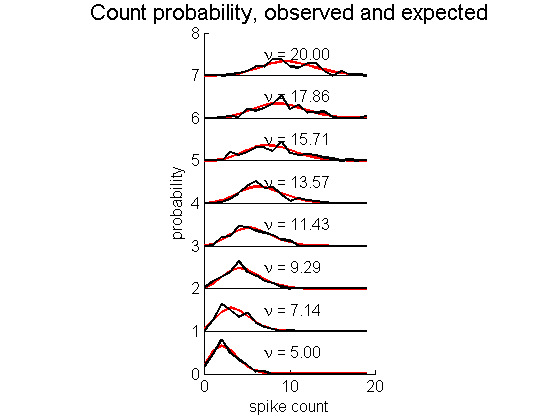
\includegraphics[trim = {1.3cm 0 1.5cm 0.1cm}, width=0.6\textwidth, clip]{../pics/as1}
\caption{The observed (black) and expected (red) count probability for the different conditions. The observed probabilities fit fairly well to the expected values. The differences can be attributed to the comparatively low number of samples used (100) and vanish with higher sample sizes.}
\label{as1}
\end{figure}

\section{Assignment III: identification performance}

We computed the reliability of correctly identifying the stimulus condition and compared the results to the theoretical value. Initial results are shown in Figure \ref{as3}. The theoretical and empirical results do not fit well together. In particular, the theoretical reliability peaks at $t=0.8\si{s}$, which does not make sense, because in theory, the longer you observe a Poisson process, the closer the measured spiking rate will be to the actual underlying value and you get a higher reliability. This is due to the fact, that when generating the \texttt{SpikeRaster} we set \texttt{Nspike=20}. This means, that even when there would have been more spikes before $t_0$, they are not generated and falsify the results. We repeated the calculations with \texttt{Nspike=200} to virtually guarantee, that spikes are never stopped generating prematurely. The results are shown in Figure \ref{as32}. As expected, the fraction correct now increases with time. The analytical solution is however higher than the empirical one, by what looks to be a constant factor. The reason for this is, that the empirical and the analytical solutions do not use consistent methods to calculate the fraction of correct identifications. A non-technical possible explanation could be, that for the theoretical calculation, all of the available information is concentrated into the single most likely result, whereas with the formula used for the empirical values the available information is distributed evenly among all candidates.

\begin{figure}
\centering
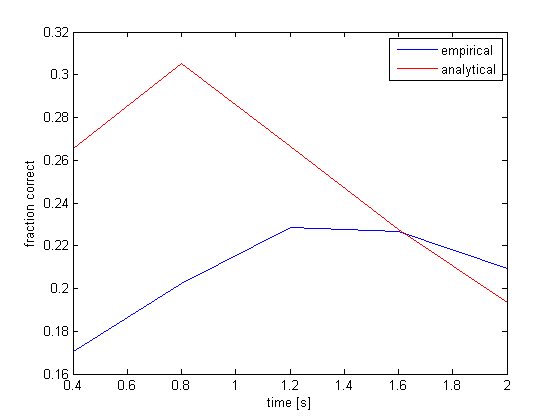
\includegraphics[trim = {0.6cm 0 1.2cm 0.7cm}, width=0.7\textwidth, clip]{../pics/as3}
\caption{The empirical (blue) and theoretical (red) fraction of correct identifications of the condition given a spike count, for \texttt{Nspike=20} and different values of $t_0$.}
\label{as3}
\end{figure}

\begin{figure}
\centering
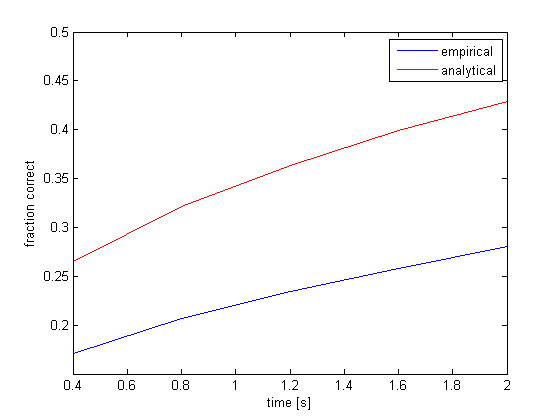
\includegraphics[trim = {0.6cm 0 1.2cm 0.7cm}, width=0.7\textwidth, clip]{../pics/as3_2}
\caption{The empirical (blue) and theoretical (red) fraction of correct identifications of the condition given a spike count, for \texttt{Nspike=200} and different values of $t_0$.}
\label{as32}
\end{figure}

\section*{Addendum}

Everything written above is what I managed to finish on time before I had to submit the exercise. For the time being, I will leave it as it is, and take the time here to explain why assignment III is some major bullshit. Admittedly, I did not pay attention during the tutorial, where some of the intricacies of this exercise sheet may have been explained, but having a tutorial and a consultation hour does not excuse shitty settings of tasks.
\subsection*{Number of spikes}
Nowhere in the entire exercise sheet are you explicitly told which value to choose for \texttt{Nspike}. Implicitly it says to set \texttt{Nspike=20}. For the first exercise this is no problem whatsoever, since we only look at times smaller than 0.5\si{s}. In the third exercise this would in principle also work, if \texttt{IdentificationPerformance()}, the function that is supposed to calculate the theoretical value for the reliability, took into account, that it is only looking at a limited number of possible results. Heck, it even takes the range of possible spike counts as an argument, but then proceeds to completely ignore the fact, that there is not an infinite range of possible outcomes. To be fair to the function, this would not be a significant problem if the \texttt{Nspike} parameter had been set properly, but then again, relying on the user's intelligence is seldom a good idea.

\subsection*{Computing the reliability}
From the exercise sheet:
\begin{quote}
The mutual information quantifies the \textit{multiplicative reduction} in the number of possible stimulus conditions, given an observed spike count. Specifically, the average number of remaining possibilities, given a spike count, is $N_\mathrm{remaining} = \frac{N_\mathrm{condition}}{2^{I_m}}$. The reliability (fraction correct) of identifying stimulus condition from an observed spike count will therefore be $f_\mathrm{identify} = \frac{1}{N_\mathrm{remaining}} = \frac{2^{I_m}}{N_\mathrm{condition}}$
\end{quote}
To me, this makes intuitive sense. The mutual information lets me eliminate some of the possibilities, and then the remaining possibilities are evenly distributed, hence $\frac{1}{N_\mathrm{remaining}}$. However, the person who implemented \texttt{IdentificationPerformance()} used a different formula to calculate the reliability, which makes even more sense, and proves the formula above wrong. Take a conditional probability distribution over X given Y $P(X|Y)$ and assume you want to guess the X correctly as often as possible. So for every possible value of $Y$, you would always guess the $x$ with the highest likelihood. So let $x_y=\arg\max_x P(X=x|Y=y)$, then whenever $Y=y$, you have a probability of $P(x_y|Y=y)$ of guessing correctly. To get the overall fraction of correct guesses simply sum all conditional likelihoods, weighted with the probability of the respective $y$ occurring, i.e. $f_\mathrm{identify}=\sum_y P(x_y|Y=y) \cdot P(Y=y)$. A simple example shows that this is not equivalent to the formula above.

Consider the joint distribution of two random variables $X$ and $Y$ given in Table \ref{ex}. As can be easily verified, $H(X) = H(Y) = 1$, $H(X,Y) = 1.7219$ and $I_m = H(X) + H(Y) - H(X, Y) = 0.2781$. According to the first formula $f_\mathrm{identify}=0.6063$. Using common sense and/or the second formula $f_\mathrm{identify}=0.8$. Whenever $Y=y_1$ guess $X=x_1$, whenever $Y=y_2$ guess $X=x_2$ and you will have on average 80\% correct.

\begin{table}
\centering
\begin{tabular}{c | c c | c}
$P(X, Y)$ & $y_1$ & $y_2$ & $P(X)$ \\  \hline
$x_1$ & 0.4 & 0.1 & 0.5 \\
$x_2$ & 0.1 & 0.4 & 0.5 \\ \hline 
$P(Y)$ & 0.5 & 0.5 &
\end{tabular}
\caption{A simple example distribution, that shows that the two formulas are not equivalent.}
\label{ex}
\end{table}

Now the question is, why the first formula does not work. I suspect it may be related to the difference between being scored on how often you are correct (where you should always bet on whichever outcome has the highest probability) versus being scored on how accurate your credence is, i.e. you say which probability distribution you expect, and get scored on how close to the real distribution you are.

\end{document}